\documentclass{article}

% if you need to pass options to natbib, use, e.g.:
% \PassOptionsToPackage{numbers, compress}{natbib}
% before loading nips_2018

% ready for submission
\usepackage[nonatbib]{nips_2018}

% to compile a preprint version, e.g., for submission to arXiv, add
% add the [preprint] option:
% \usepackage[preprint]{nips_2018}

% to compile a camera-ready version, add the [final] option, e.g.:
% \usepackage[final]{nips_2018}

% to avoid loading the natbib package, add option nonatbib:

\usepackage[utf8]{inputenc} % allow utf-8 input
\usepackage[T1]{fontenc}    % use 8-bit T1 fonts
\usepackage{hyperref}       % hyperlinks
\usepackage{url}            % simple URL typesetting
\usepackage{booktabs}       % professional-quality tables
\usepackage{amsfonts}       % blackboard math symbols
\usepackage{cite}

% The \author macro works with any number of authors. There are
% two
% commands used to separate the names and addresses of multiple
% authors: \And and \AND.
%
% Using \And between authors leaves it to LaTeX to determine where to
% break the lines. Using \AND forces a line break at that point. So,
% if LaTeX puts 3 of 4 authors names on the first line, and the last
% on the second line, try using \AND instead of \And before the third
% author name.
\usepackage{amssymb}
\usepackage{amsmath,amsthm}
\usepackage{float}
\usepackage{url}
\usepackage{setspace}
\usepackage{hyperref}
\usepackage{todonotes}
\usepackage{amsthm} 
\usepackage[ruled,vlined,linesnumbered]{algorithm2e} 
\usepackage{makecell}
\usepackage{upgreek}
\onehalfspacing
\usepackage{pdfpages}
\usepackage{times}
\usepackage{multirow}
\usepackage[toc,page]{appendix}
\usepackage{listings}
\newtheorem{thm}{Theorem}
\newtheorem{lemma}[thm]{Lemma}
\newtheorem{definition}[thm]{Definition}
\newtheorem{observation}[thm]{Observation}
\newtheorem{theorem}[thm]{Theorem}
\newtheorem{claim}[thm]{Claim}
\newtheorem{example}[thm]{Example}
\newtheorem{proposition}[thm]{Proposition}
\newtheorem{corollary}[thm]{Corollary}
\usepackage{color,soul}
\usepackage{tikz}
\usetikzlibrary{arrows,shapes.geometric,shapes.arrows}
\usepackage{pgfplots}
\usepackage{multirow}


\DeclareMathOperator{\supp}{support}
\DeclareMathOperator{\support}{support}
\DeclareMathOperator{\Trim}{Trim}
\DeclareMathOperator{\LTrim}{LTrim}
\SetKwFunction{mEqOne}{mEqOne} 
\DeclareMathOperator{\KlmApprox}{KolmogorovApprox}
%\DeclareMathOperator{\OptTrim}{KolmogorovApprox}
\DeclareMathOperator{\OptTrim}{OptTrim}


%\title{An algorithm for Kolmogorov distance based approximation of discrete random variables}
\title{A Kolmogorov-distance based approximation of discrete random variables}

\begin{document}
	
	
	\maketitle
	\begin{abstract}
		We present an algorithm that takes a discrete random variable $X$ and a number $m$ and computes a random variable whose support (set of possible outcomes) is of size at most $m$ and whose Kolmogorov distance from $X$ is minimal. In addition to a formal theoretical analysis of the correctness and of the computational complexity of the algorithm, we present a detailed empirical evaluation that shows how the proposed approach performs in practice in different applications and domains.
	\end{abstract}
	
	
	\section{Introduction}
	
	Many different approaches to approximation of probability distributions are studied in the literature~\cite{AMCR83,pavlikov2016cvar,PS77}. 
	The approaches vary in the types random variables considered, how they are represented, and in the criteria used for evaluation of the quality of the approximations. This paper is on approximating discrete distributions represented as explicit probability mass functions with ones that are simpler to store and to manipulate. This is needed, for example, when a discrete distribution is given as a large data-set, obtained, e.g., by sampling, and we want to represent it approximately with a small table (see~\cite{huq2016efficient} for example).  
	
	The main contribution of this paper is an efficient algorithm for computing the best possible approximation of a given random variable with a random variable whose complexity is not above a prescribed threshold, where the measures of the quality of the approximation and the complexity of the random variable are as specified in the following two paragraphs. 
	
	We measure the quality of an approximation by the distance between the original variable and the approximate one. Specifically, we use the Kolmogorov distance which is  commonly used for comparing random variables in statistical practice and literature. Given two random variables $X$ and $X'$ whose cumulative distribution functions (cdf) are $F_X$ and $F_{X'}$, respectively, the Kolmogorov distance between $X$ and $X'$ is $d_K(X,X')= \sup_t |F_X(t) - F_{X'}(t)|$ (see, e.g.,~\cite{gibbons2011nonparametric}). We say that $X'$ is a good approximation of $X$ if $d_K(X,X')$ is small.
	
	The complexity of a random variable is measured by the size of its support, the number of values that it can take, $|\support(X)|=|\{x\colon Pr(X=x) \neq 0\}|$. When distributions are maintained as explicit tables, as done in many implementations of statistical software, the size of the support of a variable is proportional to the amount of memory needed to store it and to the complexity of the computations around it. In summary, the exact notion of optimality of the approximation targeted in this paper is:
	\begin{definition}
		A random variable $X'$ is an optimal $m$-approximation of a random variable $X$ if $|\support(X')| \leq m$ and there is no random variable $X''$ such that $|\support(X'')| \leq m$ and $d_K(X,X'') < d_K(X,X')$.
	\end{definition}
	
	The main contribution of the paper is an efficient algorithm that takes $X$ and $m$ as parameters and constructs an optimal $m$-approximation of $X$.
	
	%\begin{theorem} \label{thm:main}
	%	Given a random variable $X$ and a number $m$, there is an algorithm with memory and time complexity $O(|\support(X)|^2 \cdot m)$  that computes an optimal $m$-approximation of $X$.
	%\end{theorem}
	
	The rest of the paper is organized as follows. In Section~\ref{sec:rel-work} we describe how our work relates to other algorithms and problems studied in the literature. In Section~\ref{sec:alg} we detail the proposed algorithm, analyze its properties, and prove the main theorem. In Section~\ref{sec:exp} we demonstrate how the proposed approach performs on the problem of estimating the probability of hitting deadlines is plans and compare it to alternatives approximation approaches from the literature. We also demonstrate the performance of our approximation algorithm on some randomly generated random variables. The paper is concluded with a discussion in Section~\ref{sec:discussion}.
	
	\section{Related work}
	\label{sec:rel-work}
	The most relevant work related to this paper is the papers by Cohen at. al.~\cite{cohen2015estimating,CohenGW18}. These papers study approximations of random variables in the context of estimating deadlines. In this context, $X'$ is defined to be a good approximation of $X$ if $F_{X'}(t) > F_{X}(t)$ for any $t$ and $\sup_t F_{X'}(t) - F_{X}(t)$ is small. This is not a distance because it is not symmetric. The motivation given by Cohen at. al. for using this type of approximation is for cases where overestimation of the probability of missing a deadline is acceptable but underestimation is not. In Section~\ref{sec:exp}, we consider the same examples examined by Cohen at. al. and show how the algorithm proposed in this paper performs relative to the algorithms proposed there when both over- and under- estimations are allowed. As expected, the Kolmogorov distance between the approximation and the original random variable is smaller by a factor of one half, on average, when using the algorithm proposed here. 
	
	
	Another relevant prior work is the theory of Sparse Approximation (aka Sparse Representation) that deals with sparse solutions for systems of linear equations, as follows. 
	
	Given a matrix $D \in \mathbb{R}^{n \times p}$ and a vector $x \in \mathbb{R}^n$, the most studied sparse representation problem is finding the sparsest possible representation $\alpha \in \mathbb{R}^p$ satisfying $x = D\alpha$:
	\[
	\min_{\alpha \in \mathbb{R}^p} \|\alpha\|_0 \text{ subject to } x = D\alpha.
	\]
	where $\|\alpha\|_0 = |\{ i : \alpha_i \neq 0, \, i=1,\ldots,p \}|$ is the $\ell_0$ pseudo-norm, counting the number of non-zero coordinates of $\alpha$. This problem is known to be NP-Hard with a reduction to NP-complete subset selection problems.
	
	In these terms, using also the $\ell_\infty$ norm that represents the maximal coordinate and the $\ell_1$ norm that represents the sum of the coordinates, our problem can be phrased as:
	\[
	\min_{\alpha \in [0,\infty)^p}\|x - D\alpha\|_{\infty} \text{ subject to }  \|\alpha\|_0 = m \text{ and } \|\alpha\|_1=1.
	\]
	where $D$ is the all-ones triangular matrix (the entry at row $i$ and column $j$ is one if $i\leq j$ and zero otherwise), $x$ is related to $X$ such that the $i$th coordinate of $x$ is $F_X(x_i)$ where $\support(X)=\{x_1 < x_2 < \cdots < x_n\}$ and $\alpha$ is related to $X'$ such that the $i$th coordinate of $\alpha$ is $f_{X'}(x_i)$. The functions $F_X$ and $f_{X'}$ represent, respectively, the cumulative distribution function of $X$ and the mass distribution function of $X'$. This, of course, means that the coordinates of $x$ are assumed to be positive and monotonically increasing and that the last coordinate of $x$ is assumed to be one. We demonstrate an application for this specific sparse representation problem and show that it can be solve in $O(n^2m)$ time and $O(m^2)$ memory.
	
	The presented work is also related to the research on binning in statistical inference. Consider, for example, the problem of credit scoring~\cite{zeng2017comparison} that deals with separating good applicants from bad applicants where the Kolmogorov–Smirnov statistic KS is a standard measure. The KS comparison is often preceded by a procedure called binning where a large table is translated to a smaller one by collecting nearby values together. There are many methods for binning~\cite{mays2001handbook,refaat2011credit,bolton2010logistic,siddiqi2012credit}.
	In this context, our algorithm can be consider as a new binning strategy that provides optimality guarantees with respect to the Kolmogorov distance that none of the existing binning technique that we are aware of provides.
	
	The present study is also related to the work of Pavlikov and Uryasev~\cite{pavlikov2016cvar}, where a procedure for producing a random variable $X'$ that optimally approximates a random variable $X$ is presented. Their approximation scheme, achieved using linear programming, is designed for a different notion of distance (called CVaR). The new contribution of the present work in this context is that our method is direct, not using linear programming, thus allowing tighter analysis of time and memory complexity. Also, our method is designed for optimizing the Kolmogorov distance that is more prevalent in applications. For comparison, in Section~\ref{sec:exp} we briefly discuss the performance of linear programming approach similar to the one proposed in~\cite{pavlikov2016cvar} for the Kolmogorov distance and compare it to the algorithm proposed in this paper. 
	
	\section{An algorithm for optimal approximation}\label{sec:alg}
	In the scope of this section, let $X$ be a given random variable with a finite support of size $n$, and let  $0<m\leq n$ be a given complexity bound. The section evolves by developing notations and by collecting facts towards an algorithm for finding an optimal $m$-approximation of $X$.
	
	The first useful fact is that it is enough to limit our search to approximations $X'$s such that $\support(X') \subseteq \support(X)$:
	
	\begin{lemma}\label{lem:supContained}
		For every random variable $X''$ there is a random variable $X'$ such that $\support(X') \subseteq \support(X)$ and $d_{K}(X,X')\leq d_{K}(X,X'')$.
	\end{lemma}
	
	\begin{proof}
		Let $\{x_1,\dots,x_n\} = \support(X)$, and let $x_0 = -\infty, x_{n+1}=\infty$. Consider the random variable $X'$ whose probability mass function is
		$f_{X'}(x_i) = P(x_{i-1} < X'' \leq x_i)$ for $i=1,\dots,n-1$,  $f_{X'}(x_n) = P(x_n-1 < X'' < x_{n+1})$, and $F_{X'}(x)=0$ if $x\notin \support(X)$.  Since $X'$ only "pushes" the probability mass of $X''$ to the support of $X$, we have that $f_{X'}$ is a probability mass function and therefore $X'$ is well defined. 	
		By construction, $|F_{X}(x_i)-F_{X'}(x_i)| = |F_{X}(x_i)-F_{X''}(x_i)|$ for every  $1\leq i\leq n-1$. For $i=n$ we have $|F_{X}(x_n)-F_{X'}(x_n)| = |1-1|=0$.
		Since $|F_{X}(x)-F_{X'}(x)| = |F_{X}(x_i)-F_{X'}(x_i)|$ for every  $0\leq   i < n+1$  and $x_i<x<x_{i+1}$, we have that $d_K(X,X')=max_{i}|F_{X}(x_i)-F_{X'}(x_i)|\leq max_{i}|F_{X}(x_i)-F_{X''}(x_i)|\leq d_K(X,X'')$.
	\end{proof}
	
	%Next, note that every random variable $X''$ with support of size at most $m$ that is contained in $\support(X)$ can be described by first setting the (at most $m$) elements of the support of $X''$; then for every such option, determine $X''$ by setting probability values for the elements in the chosen support of $X'$, and setting $0$ for rest of the elements.
	
	For a set $S\subseteq \support(X)$, let $\mathbb{X}_S$ denote the set of random variables whose supports are contained in $S$. In Step 1 below, we find a random variable in $\mathbb{X}_S$  that minimizes the Kolmogorov distance from $X$. We denote the Kolmogorov distance between this variable and $X$ by $\varepsilon(X,S)$. Then, in Step 2, we show how to efficiently find a set $S \subseteq \support(X)$ whose size is smaller or equal to $m$ that minimizes $\varepsilon(X,S)$. Then, in Step 3, an optimal $m$-approximation is constructed by taking a minimal approximation in $\mathbb{X_S}$ where $S$ is the set that that minimizes $\varepsilon(X,S)$. 
	
	\subsection*{Step 1: Finding an $X'$ in $\mathbb{X}_S$ that minimizes $d_K(X,X')$}
	
	
	We first fix a set $S\subseteq \support(X)$ of size at most $m$, and among all the random variables in $\mathbb{X}_S$ find one with a minimal distance from $X$. Denote the elements of $S$ in increasing order by $S=\{x_1<\dots<x_m\}$ and let $x_0=-\infty$ and $x_{m+1}=\infty$. For every $1 <  i \leq m$ let $\hat x_i$ be the maximal element of $\support(X)$ that is smaller than $x_i$. Consider the following weight function 
	
	\begin{definition}\label{def:weight} For $0\leq i \leq m$ let
		\[
		w(x_i,x_{i+1})=
		\begin{cases}
		P(x_i < X < x_{i+1}) & \text{if $i=0$ or $i = m$;} \\
		P(x_i < X < x_{i+1})/2 & \text{otherwise.} \\	
		\end{cases}
		\]
	\end{definition}
	
	Note that $P(x_i < X < x_{i+1}) = F_X(\hat x_{i+1}) - F_X(x_i)$, a fact that we will use throughout this section.
	
	\begin{definition}\label{def:error}
		Let $\varepsilon(X,S) = \max\limits_{i=0,\dots,m} w(x_{i}, x_{i+1})$.
	\end{definition}
	
	
	
	We first show that $\varepsilon(X,S)$ is a lower bound for the distance between random variable in $\mathbb{X}_S$ and $X$. Then, we present a random variable $X'\in \mathbb{X}_S$ such that $d_K(X,X')=\varepsilon(X,S)$. It then follows that $X'$ is an optimal $m$-approximation random variable among all random variables in $\mathbb{X}_S$.
	
	%The intuition behind choosing these specific weights and $\varepsilon(X,S)$ being a lower bound is as follows.  Since for every $X'\in\mathbb{X}_S$ the probability mass of $X'$ for the elements not in $S$ are set to $0$, we have that $F_{X'}(\hat x_{i+1})=F_{X'}(x_i)$. Therefore the distance between $X'$ and $X$ at points $x_i$ and $\hat x_{i+1}$ that we have to take into additional account is increased by $F_X(\hat x_{i+1})-F_X(x_i) = P(x_i < X < x_{i+1})$.
	
	%Formally we have the following.
	
	\begin{proposition}\label{prop:minimal}
		If $X'\in\mathbb{X}_S$ then $d_K(X,X') \geq \varepsilon(X,S)$.
	\end{proposition}
	
	\begin{proof}
		
		
		By definition, for every $0\leq i\leq m$, $d_K(X,X') \geq \max \{|F_X(\hat x_{i+1}) - F_{X'}(\hat x_{i+1})|,|F_X(x_i) - F_{X'}(x_i)| \}$. Note that $F_{X'}(\hat x_{i+1})=F_{X'}(x_i)$ since the probability values for all the elements not in $S$ are set to $0$.
		
		If $i=0$, that is $x_i=-\infty$, we have that $F_X(x_i)=F_{X'}(x_i)=F_{X'}(\hat x_{i+1})=0$ and therefore $d_K(X,X') \geq |F_X(\hat x_{i+1})| = |F_X(\hat x_{i+1}) - F_{X}(x_i)| =  P(x_i < X < x_{i+1})= w(x_i,x_{i+1})$.
		
		If $i =m$, that is $x_{i+1}=\infty$, we have that $F_X(\hat x_{i+1})=F_{X'}(\hat x_{i+1})=F_{X'}(x_i)=1$. 
		and therefore $d_K(X,X') \geq |1-F_X(\hat x_i)| = |F_X(\hat x_{i+1}) - F_{X}(x_i)| =  P(x_i < X < x_{i+1}) = w(x_i,x_{i+1})$. 
		
		%  we have that $F_X(x_i)=F_{X'}(x_i)=F_{X'}(\hat x_{i+1})=0$ 
		% 
		% 
		% 
		% We break the proof for the closed intervals where each support variable $x_i$ is a proper number, and for the open intervals where a support variable is either $-\infty$ or $\infty$.
		
		Otherwise for every $1\leq i< m$,  we use the fact that $max\{|a|,|b|\} \geq |a-b|/2$ for every $a,b\in\mathbb{R}$, to deduce that $d_K(X,X') \geq 1/2| F_X(\hat x_{i+1}) - F_X(x_i) + F_{X'}(x_i) -F_{X'}(\hat x_{i+1})|$. So $d_K(X,X') \geq 1/2| F_X(\hat x_{i+1}) - F_X(x_i) | =P(x_1 < X < x_2)/2 = w(x_i,x_{i+1})$. 
		
		Since $d_K(X,X') \geq  w(x_i,x_{i+1})$ for every $0\leq i\leq m$, the proof follows by the definition of $\varepsilon(X,S)$.
	\end{proof}
	
	
	
	Next we describe a random variable $X'\in\mathbb{X}_S$ with a distance of $\varepsilon(X,S)$ from $X$. Thus $X'$ is an optimal $m$-approximation among the set $\mathbb{X}_S$. The variable $X'$ is described by its probability mass function:
	
	\begin{definition}\label{def:construction}
		Let $f_{X'}(x_{i}) = w(x_{i-1},x_i) + w(x_i,x_{i+1}) + f_{X}(x_i)$ for $i=1,\dots,m$ and $f_{X'}(x)=0$ for $x \notin S$.
	\end{definition}
	
	We first show that $X'$ is a properly defined random variable:
	
	\begin{lemma}
		$f_{X'}$ is a probability mass function. 
	\end{lemma}
	
	\begin{proof}
		From definition $f_{X'}(x_{i})\geq 0$ for every $i$. To see that $\sum_i f_{X'}(x_{i}) =1$, 
		we have $\sum_i f_{X'}(x_{i}) = \sum_i (w(x_{i-1},x_i) + w(x_i,x_{i+1}) + f_{X}(x_i)) = 	
		\sum _{x_i\in S} f_{X}(x_i)) + w(x_0,x_1)+ \sum_{0 < i < m} 2 w(x_i,x_{i+1}) + w(x_m,x_{m+1}) = 
		\sum _{x_i\in S} P(X{=}x_i) + P(x_0 {<} X {<} x_1)+ \sum_{0 < i < m} P(x_i < X < x_{i+1}) +P(x_m < X < x_{m+1}) = 1$ since this is the entire support of $X$.	
	\end{proof}
	
	
	Note that $X'$ can be constructed in time linear in the size of the support of $X$. %Intuitively the setting of $X'$ allows to take an "advantage" of distance from $X$ at the elements of $\support(X')$, to avoid the overall increased distance of $X$ from $X'$ at the elements that are not at $\support(X)$ and in which $f_{X'}$ is set to $0$. Formally we have the following.
	Its main property, of course, the distance between the cumulative distribution functions of $X$ and $X'$ are bounded by $w(x_i,x_{i+1})$, as follows:
	\begin{lemma}\label{lem:balance}
		Let $x\in\support(X)$ and $0\leq i\leq m$ be such that $x_i\leq x \leq x_{i+1}$ then $-w(x_i,x_{i+1})\leq F_X(x)-F_{X'}(x)\leq  w(x_i,x_{i+1})$.
	\end{lemma}
	
	\begin{proof}	
		
		We prove by induction on $0\leq i < m$ .
		
		First see that $F_{X'}(j) = 0$  for every $x_0<j < x_1$ and therefore $F_X(j)-F_{X'}(j) = F_X(j)-0 \leq F_X(\hat x_1)= F_X(\hat x_1)- F_X(x_0) = w(x_0,x_1)$. For $ j = x_1$ we have $F_X(x_1)-F_{X'}(x_1)=  F_X(\hat x_1) +f_{X}(x_1) - (w(x_0,x_1) + w(x_1,x_2) + f_{X}(x_1) = 
		w(x_0,x_1) +f_{X}(x_1) - (w(x_0,x_1) + w(x_1,x_2) + f_{X}(x_1)) = -w(x_1,x_2)$.
		
		Next assume that $F_X(\hat x_i)-F_{X'}(\hat x_i) = w(x_{i-1},x_i)$.
		Then $F_X(x_i)-F_{X'}(x_i) =  F_X(\hat x_i) +f_{X}(x_i) - (w(x_{i-1},x_i) + w(x_i,x_{i+1}) + f_{X}(x_i)) =  w(x_{i-1},x_i) +f_{X}(x_{i}) - (w(x_{i-1},x_i) + w(x_{i},x_{i+1}) + f_{X}(x_{i})) = -w(x_{i},x_{i+1})$.
		
		As before we have that for all $x_i< j< x_{i+1}$, we have $F_X(j)-F_{X'}(j) = F_X(j)-F_{X'}(\hat x_{i+1}) \leq  F_X(\hat x_{i+1})-F_{X'}(\hat x_{i+1})$. Then $F_X(\hat x_{i+1})-F_{X'}(\hat x_{i+1}) = (F_X(x_i)+ P(x_i < x <x_{i+1})) - F_{X'}(x_i) = -w(x_{i},x_{i+1}) + 2w(x_{i},x_{i+1}) = w(x_{i},x_{i+1}) $.
		
		
		Finally for $x_m\leq j \leq x_{m+1}$ we have that $F_{X'}(x_m)=1$ therefore $F_X(x_m)-F_{X'}(x_m) = (1- P(x_m<X < x_{m+1})) - 1 =  P(x_m<X < x_{m+1}) = w(x_m,x_{m+1})$, and for every $x_m<j<x_{m+1}$ we have $F_X(j) - F_{X'}(j) < (1- P(x_m<X < x_{m+1})) - 1 <  - P(x_m<X < x_{m+1}))  = -w(x_m,x_{m+1})$ as required.
	\end{proof}
	
	From Lemma \ref{lem:balance}, by the definition of $\varepsilon(X,S)$, we then have:
	\begin{corollary} \label{col:Xprime}
		$d_K(X,X') = \varepsilon(X,S)$.
	\end{corollary}
	From Proposition~\ref{prop:minimal} we also have:
	\begin{corollary} \label{col:Xprimeopt}
		$\varepsilon(X,S)$ is the distance between $X$ and the variable closest to it in $\mathbb{X}_S$.
	\end{corollary}
	
	%\begin{proof}
	%	We first see by induction that for every $1\leq i \leq m$ that $F_X(\hat x_i)-F_{X'}(\hat x_i)=w(x_{i-1},x_i)$ and $F_X(x_i)-F_{X'}(x_i) = -w(x_i,x_{i+1})$. 
	%	
	%	For $i=1$ we have  $F_X(\hat x_1)-F_{X'}(\hat x_1)= F_X(\hat x_1)-0 =  F_X(\hat x_1)- F_X(x_0) = w(x_0,x_1)$.
	%	Then $F_X(x_i)-F_{X'}(x_i)=  F_X(\hat x_1) +f_{X}(x_1) - (w(x_0,x_1) + w(x_1,x_2) + f_{X}(x_1)| = 
	%	w(x_0,x_1) +f_{X}(x_1) - (w(x_0,x_1) + w(x_1,x_2) + f_{X}(x_1)) = -w(x_1,x_2)$.
	%	
	%	Assume that $F_X(x_i)-F_{X'}(x_i) = -w(x_i,x_{i+1})$. Then $F_X(\hat x_{i+1})-F_{X'}(\hat x_{i}) = (F_X(x_i)+ P(x_i<X<x_{i+1}))-F_{X'}(x_i) = -w(x_i,x_{i+1})+2w(x_i,x_{i+1})=w(x_i,x_{i+1})$.
	%	Therefore, we have $F_X(x_{i+1})-F_{X'}(x_{i+1}) = F_X(\hat x_{i+1}) +f_{X}(x_{i+1}) - (w(x_i,x_{i+1}) + w(x_{i+1},x_{i+2}) + f_{X}(x_{i+1})| = 
	%	w(x_i,x_{i+1}) +f_{X}(x_{i+1}) - (w(x_i,x_{i+1}) + w(x_{i+1},x_{i+2}) + f_{X}(x_{i+1})) = -w(x_{i+1},x_{i+2})$.
	%	
	%	
	%	[[DF: read again and see if special instructions are required for $i=0,m$, the last one]]
	%	
	%	
	%	Finally see that for every $x_i<j< x_{i+1}\in \support(X)$, $F_{X'}(j)= F_{X'}(x_i) = F_{X'}(\hat x_{i+1}) $ and therefore  $-w(x_i,x_{i+1}) = F_X(x_i)-F_{X'}(x_i) \leq F_X(j)-F_{X'}(j)\leq F_X(\hat x_{i+1})-F_{X'}(\hat x_{i+1}) = w(x_i,x_{i+1})$. Therefore $|F_X(j)-F_{X'}(j)|\leq w(x_i,x_{i+1})$.
	%	
	%	Therefore for every $j\in \support(X)$ we have that $|F_X(j)-F_{X'}(j)|\leq max_i(w(x_i,x_{i+1})=\varepsilon(X,S)$. as required.	
	%\end{proof}
	
	
	
	
	%\begin{itemize}
	%	\item The next lemma states a lower bound on the distance $d_K(X,X')$ when a range of elements is excluded from the support of $X'$.
	%\end{itemize}
	%
	%
	%\begin{lemma}\label{lem:geq}
	%	For $x_1, x_2 \in \support(X) \cup \{-\infty,\infty\}$ such that $x_1 < x_2$, if $P(x_1 < X' < x_2)=0$  then 
	%	$d_k(X,X') \geq P(x_1 < X < x_2)/2$.
	%\end{lemma}
	%\begin{proof}
	%	Let $\hat x=\max \{x \in \support(X) \cap\{ -\infty, \infty\}  \colon x < x_2 \}$. By definition, $d_k(X,X') \geq \max \{|F_X(x_1) - F_{X'}(x_1)|, |F_X(\hat x) - F_{X'}(\hat x)| \}$. From Observation~\ref{obs:ab}, $d_k(X,X') \geq 1/2|F_X(x_1) - F_X(\hat x) + F_{X'}(\hat x) - F_{X'}(x_1)|$. Since it is given that $F_{X'}(\hat x) - F_{X'}(x_1) = P(x_1 < X' < x_2)=0$, $d_k(X,X') \geq 1/2|F_X(x_1) - F_X(\hat x) | =  P(x_1 < X \leq \hat x)/2 = P(x_1 < X < x_2)/2$.
	%\end{proof}
	%
	%
	%\begin{itemize}
	%	\item The next lemma strengthen the lower bound.
	%\end{itemize}
	%
	%
	%\begin{lemma}\label{lem:geq2}
	%	For $x_1, x_2 \in \support(X) \cup \{-\infty,\infty\}$ such that $x_1=-\infty$ or  $x_2=\infty$, if $P(x_1 < X' < x_2)=0$  then 
	%	$d_k(X,X') \geq P(x_1 < X < x_2)$.
	%\end{lemma}
	%\begin{proof}
	%	Let $\hat x=\max \{x \in \support(X) \cap\{ -\infty, \infty\}  \colon x < x_2 \}$. By definition $d_k(X,X') \geq \max \{|F_X(x_1) - F_{X'}(x_1)|, |F_X(\hat x) - F_{X'}(\hat x)| \}$. If $x_1=-\infty$ then $d_k(X,X') \geq \{|F_X(\hat x) - F_{X'}(\hat x)| \}$ since $F_X(-\infty) = F_{X'}(-\infty) = 0$. Furthermore, $F_{X'}(\hat x) = P(x_1 < X' < x_2)=0$. Therefore $d_k(X,X') \geq F_X(\hat x) = P(x_1 < X \leq \hat x) = P(x_1 < X < x_2)$. 
	%	If $x_2=\infty$ then $d_k(X,X') \geq \{|F_X(x_1) - F_{X'}(x_1)| \}$ since $F_X(\hat{x}) = F_{X'}(\hat{x}) = F_X(\infty) = F_{X'}(\infty) = 1$. Furthermore, $F_{X'}(x_1) = 1$ since it is given that $P(x_1 < X' < x_2)=0$. Therefore we get that $d_k(X,X') \geq |F_X(x_1)-1| = |1-F_X(\hat x)-| = P(x_1 < X \leq \hat x) = P(x_1 < X < x_2)$.
	%\end{proof}
	%
	%
	%\begin{definition}\label{def:weight} For $x_1,x_2 \in \support(X) \cup \{-\infty,\infty\}$ let
	%	\[
	%	w(x_1,x_2)=
	%	\begin{cases}
	%	P(x_1 < X < x_2) & \text{if $x_1=-\infty$ or $x_2 = \infty$;} \\
	%	P(x_1 < X < x_2)/2 & \text{otherwise.} \\	
	%	\end{cases}
	%	\]
	%\end{definition} 
	%
	%
	%\begin{definition}\label{def:error} For $S=\{x_1<\dots<x_m\} \subseteq \support(X)$, $x_0=-\infty$, and $x_{m+1}=\infty$, let
	%	\[
	%	\varepsilon(X,S) = \max\limits_{i=0,\dots,m} w(x_{i}, x_{i+1}).
	%	\]
	%\end{definition} 
	%
	%\begin{itemize}
	%	\item From here on, until the end of the section, $S$ is fixed.
	%\end{itemize}
	
	
	%
	%\begin{proposition}
	%	There is no $X'$ such that $\support(X')=S$ and $d_k(X,X') < \varepsilon(X,S)$.
	%\end{proposition}
	%\begin{proof}
	%	Let $i$ be the index that maximizes $w(x_{i}, x_{i+1})$. If $0<i<n-1$ then $d_k(X,X') \geq w(x_{i}, x_{i+1})$ by Lemma~\ref{lem:geq}. If $i=0$ or $i=n+1$ the same follows from Lemma~\ref{lem:geq2}.
	%\end{proof}
	
	
	
	
	%
	%\begin{lemma}
	%	For $i>1$, if $F_{X'}(x_{i})-F_{X}(x_{i}) = w(x_{i}, x_{i+1})$ then $F_{X'}(x_{i+1})-F_{X}(x_{i+1}) = w(x_{i+1}, x_{i+2})$.
	%\end{lemma}
	%\begin{proof}
	%	\begin{align}
	%	&F_{X'}(x_{i+1})-F_{X}(x_{i+1}) = \\ \nonumber
	%	& = f_{X'}(x_{i+1}) - f_{X}(x_{i+1}) - P(X<x_{i+1}) + P(X'<x_{i+1})  \\ \nonumber
	%	& = f_{X'}(x_{i+1}) - f_{X}(x_{i+1}) - F_X(x_{i}) - P(x_{i}< X < x_{i+1}) + F_{X'}(x_{i}) \\ 
	%	\label{eq:weight}
	%	& = f_{X'}(x_{i+1}) - f_{X}(x_{i+1}) - F_X(x_{i}) - 2w(x_{i},x_{i+1}) + F_{X'}(x_{i})  \\ \label{eq:indHip}
	%	& = f_{X'}(x_{i+1}) - f_{X}(x_{i+1}) - 2w(x_{i},x_{i+1}) +w(x_{i}, x_{i+1})  \\ \label{eq:construction}
	%	& = w(x_{i},x_{i+1}) +w(x_{i+1},x_{i+2}) - 2w(x_{i},x_{i+1}) +w(x_{i}, x_{i+1}) \\ \nonumber
	%	& = w(x_{i+1},x_{i+2}) \nonumber
	%	\end{align}
	%	
	%	By Definition~\ref{def:weight} the probability $P(x_{i-1}< X < x_i) = 2w(x_{i-1},x_{i})$ as in Equation~\eqref{eq:weight}. Equation~\eqref{eq:indHip} is deduced by the induction hypothesis and Equation~\eqref{eq:construction} where
	%	$f_{X'}(x_i) - f_{X}(x_i) = w(x_{i-1},x_i) + w(x_i,x_{i+1})$ is true by construction, see Definition\ref{def:construction}.
	%\end{proof}
	
	%\begin{lemma}
	%	For $i>1$, if $F_{X'}(x_{i-1})-F_{X}(x_{i-1}) = w(x_{i-1}, x_{i})$ then $F_{X'}(x_{i})-F_{X}(x_i) = w(x_i, x_{i+1})$.
	%\end{lemma}
	%\begin{proof}
	%	% TODO switch tdirections to fit the statement of the lemma
	%	% TODO \eqref,  aligment
	%	\begin{align}
	%	&F_X(x_i)-F_{X'}(x_i) = \\
	%	&f_{X}(x_i) - f_{X'}(x_i) + P(X<x_i) - P(X'<x_i)  = \\ \nonumber
	%	&f_{X}(x_i) - f_{X'}(x_i) + F_X(x_{i-1}) + P(x_{i-1}< X < x_i)-F_{X'}(x_{i-1}) = \\
	%	&f_{X}(x_i) - f_{X'}(x_i) + F_X(x_{i-1}) + 2w(x_{i-1},x_{i})-F_{X'}(x_{i-1}) =^* \\
	%	&f_{X}(x_i) - f_{X'}(x_i) + 2w(x_{i-1},x_{i}) -w(x_{i-1}, x_{i}) = \\
	%	& -w(x_{i-1},x_i) - w(x_i,x_{i+1}) + 2w(x_{i-1},x_{i}) -w(x_{i-1}, x_{i}) =\\ 
	%	&- w(x_i,x_{i+1})
	%	\end{align}
	%	$*$ by induction hypothesis.
	%	The probability $P(x_{i-1}< X < x_i) = 2w(x_{i-1},x_{i})$ by Definition~\ref{def:weight}, and
	%	$f_{X'}(x_i) - f_{X}(x_i) = w(x_{i-1},x_i) + w(x_i,x_{i+1})$ by construction.
	%\end{proof}
	%
	%\begin{lemma}
	%	Base case: $i = 1, F_{X'}(x_{1})-F_{X}(x_{1}) = w(x_{1}, x_{2})$.
	%\end{lemma}
	%\begin{proof}
	%	\begin{align*}
	%	F_{X'}(x_{1})-F_{X}(x_{1}) &= \\
	%	& = f_{X'}(x_{1}) - f_{X}(x_{1}) - w(x_0, x_1)  \\
	%	& = w(x_{0},x_1) + w(x_1,x_{2}) - w(x_0, x_1)  \\
	%	& = w(x_1,x_{2})
	%	\end{align*}
	%\end{proof}
	%
	%
	%
	
	
	%\begin{proof}
	%	Define $X'$ to by $f_{X'}(x_i) = w(x_{i-1},x_i) + w(x_i,x_{i+1}) + f_{X}(x_i)$ for $i=1,\dots,m$ and $f_{X'}(x)=0$ for $x \notin S$.
	%	We need to show that $F_X(x_i)-F_{X'}(x_i) = -w(x_i, x_{i+1})$. Assume this is true for every $j<i$, the induction hypothesis hereby: $F_X(x_{i-1})-F_{X'}(x_{i-1}) = -w(x_{i-1}, x_{i})$.
	%	\begin{align*}
	%		&F_X(x_i)-F_{X'}(x_i) = \\
	%		&f_{X}(x_i) - f_{X'}(x_i) + P(X<x_i) - P(X'<x_i)  = \\
	%		&f_{X}(x_i) - f_{X'}(x_i) + F_X(x_{i-1}) + P(x_{i-1}< X < x_i)-F_{X'}(x_{i-1}) = \\
	%		&f_{X}(x_i) - f_{X'}(x_i) + F_X(x_{i-1}) + 2w(x_{i-1},x_{i})-F_{X'}(x_{i-1}) =^* \\
	%		&f_{X}(x_i) - f_{X'}(x_i) + 2w(x_{i-1},x_{i}) -w(x_{i-1}, x_{i}) = \\
	%		& -w(x_{i-1},x_i) - w(x_i,x_{i+1}) + 2w(x_{i-1},x_{i}) -w(x_{i-1}, x_{i}) =\\ 
	%		&- w(x_i,x_{i+1})
	%	\end{align*}
	%	$*$ by induction hypothesis.
	%	The probability $P(x_{i-1}< X < x_i) = 2w(x_{i-1},x_{i})$ by definition~\ref{def:weight}, and
	%	$f_{X'}(x_i) - f_{X}(x_i) = w(x_{i-1},x_i) + w(x_i,x_{i+1})$ by construction.
	%	
	%\end{proof}
	
	
	
	%\begin{proposition}
	%	For any random variable $X$ and an ordered set $S=\{x_1<\dots<x_m\} \subset \support(X)$ there is no random variable $X'$ such that $\support(X')=S$ and $d_k(X,X') < \max\limits_{i=0,\dots,m} w(x_{i}, x_{i+1})$ where, to simplify notations, we assume that $x_0=-\infty$ and $x_{m+1}=\infty$.
	%\end{proposition}
	%
	%\begin{proof}
	%	Let $i$ be the index that maximizes $w(x_{i}, x_{i+1})$. If $0<i<n-1$ then $d_k(X,X') \geq w(x_{i}, x_{i+1})$ by Lemma~\ref{lem:geq}. If $i=0$ or $i=n+1$ the same follows from Lemma~\ref{lem:geq2}.
	%\end{proof}
	%
	%\begin{itemize}
	%	\item The next lemma shows that there is a n not better approximation. 
	%\end{itemize}
	%
	%
	%
	%\begin{proposition}
	%	For any random variable $X$ and an ordered set $S=\{x_1<\dots<x_m\} \subset \support(X)$ there is a random variable $X'$ such that $\support(X')=S$ and $d_k(X,X') = \max\limits_{i=0,\dots,m} w(x_{i}, x_{i+1})$ where, to simplify notations, we assume that $x_0=-\infty$ and $x_{m+1}=\infty$.
	%\end{proposition}
	%\begin{proof}
	%Define $X'$ to by $f_{X'}(x_i) = w(x_{i-1},x_i) + w(x_i,x_{i+1}) + f_{X}(x_i)$ for $i=1,\dots,m$ and $f_{X'}(x)=0$ for $x \notin S$.
	%\end{proof}
	
	%%%%%%%%%%%%%%%%%%%% New sec 3.2 %%%%%%%%%%%%%%%%%%%%%%%%%%%%%%%%%%%%%
	
	
	\subsection*{Step 2: Finding a set $S$ that minimizes $\varepsilon(X,S)$}
	
	We proceed to finding an $S$ that minimizes $\varepsilon(X,S)$. To obtain that we use a graph search approach motivated by a method described in~\cite{chakravarty1982partitioning}. We construct a directed graph with a source and a target in which each source-to-target path of length smaller or equal to $m$ corresponds to a possible support set of the same size, and the weights along that path correspond to the weight as defined in Definition~\ref{def:weight}. Thus the problem of finding an $S$ that minimizes $\varepsilon(X,S)$ is reduced to the problem of finding a source-to-target path $\vec{p}$ of length smaller or equal to $m$ in that graph such that the maximal weight of an edge in $\vec{p}$ is minimal among all other such maximal edges in all other such paths. 
	
	
	More specifically, the vertexes of the graph are $V=\support(X) \cup \{-\infty,\infty\}$ and the edges, $E$, are all the pairs $(x_1,x_2) \in V^2$ such that $x_1 < x_2$. The weight 
	of each edge is as specified in Definition~\ref{def:weight}. Note that there is a one-to-one correspondence between a set $S \subseteq \support(X)$ of size $m$, and an $-\infty$-to-$\infty$ path $\vec{p}_S$ in $G$, obtained by removing the $-\infty$ and $\infty$ from the path in one way and by adding these elements and the sorting on the other way. 
	With this correspondence the maximal weight of an edge on $\vec{p}_S$ is $\varepsilon(X,S)$. We denote this maximal weight of an edge  by $w(\vec{p}_S)$, and denote the set of all acyclic $-\infty$-to-$\infty$ paths in $G$ with at most $m$ edges by $paths_m(G, -\infty, \infty)$. Thus, the problem of finding the set $S$ with the minimal  $\varepsilon(X,S)$ is now reduced to the problem of finding a path $\vec{p}\in paths_m(G, -\infty, \infty)$ such that $w(\vec{p})$ is minimal among all $\{w(\vec{p'}) \colon \vec{p'}\in paths_m(G, -\infty, \infty)\}$. 
	This problem can be solved by a variant of the Bellman-Ford algorithm and by the improved algorithm described in~\cite{guerin2002computing}.
	
	
	%\begin{corollary}\label{cor:Bellman}
	%$BellmanFord(G,m)$ returns a path $\vec{p}\in paths_m(G, s, t)$ such that $w(\vec{p})$ is minimal among all $\{w(\vec{p'}) | \vec{p'}\in paths_m(G, s, t)\}$.
	%\end{corollary}
	
	
	\subsection*{Step 3: Constructing the overall algorithm}
	
	We combine Step 1 and Step 2 in the following algorithm called $\KlmApprox$ (Algorithm~\ref{alg:optapprox}) that follows naturally from the two steps. Given $X$ and $\support(X)$ we add $x_0,x_{n+1}$ and construct the graph (line 2) as in Step 2. Then we execute a variant of the Bellman-Ford algorithm on $G$ for $m$ iterations, or the algorithm proposed in~\cite{guerin2002computing}, to obtain a path $\vec{p}=(v_0,\dots,v_{m+1})$ (line 2). Finally we use Definition~\ref{def:construction} to construct $X'$ from $\vec{p}$ (lines 4-5).
	
	
	\begin{algorithm}\label{alg:optapprox}
		\DontPrintSemicolon
		Construct a weighted graph $G=(V,E)$ where $V=\support(X) \cup \{-\infty,\infty\}$, $E=\{(x_1,x_2) \in V^2\colon x_1 < x_2 \}$, and the weights are as in Definition~\ref{def:weight}.\;
		
		Find a path $\vec{p}=(x_0,\dots,x_{m+1})\in paths_m(G, -\infty, \infty)\}$ such that $w(\vec{p}) = \min \{w(\vec{p}) \colon \vec{p}\in paths_m(G, -\infty, \infty)\}$.   \;
		
		Return a random variable whose probability mass function is 
		$f_{X'}(x_{i}) = w(x_{i-1},x_i) + w(x_i,x_{i+1}) + f_{X}(x_i)$ for all $i=1,\dots,m$ and zero otherwise. \;
		
		\caption{$\KlmApprox (X, m)$}  
		\label{alg:sequence}
	\end{algorithm}
	
	
	
	%\begin{algorithm}\label{alg:optapprox}
	%	\DontPrintSemicolon
	%	\SetKwFunction{Convolv}{Conv}
	%	\SetKwFunction{getPartition}{getPartition}
	%	\SetKwFunction{bellmanFordMinMaxM}{bellmanFordMinMaxM}
	%	$\support(X)\cup \{x_0,x_{n+1}\}$\;
	%	Construct $G=(V,E,s,t,w)$ according to Step 2 \;
	%	$\vec{p}=(v_0,\dots,v_{m+1}) = Belmman-Ford(G,m)$  \;
	%	\For{$0<i<m+1$ }{
	%		$f_{X'}(x_{i}) = w(v_{i-1},v_i) + w(v_i,v_{i+1}) + f_{X}(x_i)$
	%	}	
	%	\Return $X'$\;
	%	
	%	\caption{$\KlmApprox (X, m)$}  
	%	\label{alg:sequence}
	%\end{algorithm}
	
	
	
	\begin{theorem}\label{the:algo}
		$\KlmApprox$ returns an $m$-optimal-approximation of $X$.
	\end{theorem}
	\begin{proof}
		By the construction of $G$ we get that the path $\vec{p}$ obtained in line 4 of  $\KlmApprox$ describes a set $S$ of support of size at most $m$ for which $\varepsilon(S,X)$ is minimal. Then from Definition \ref{def:construction} and Corollary \ref{col:Xprime} we construct $X'$ in lines 4-5 of 	$\KlmApprox$ such that $d_K(X,X') = \varepsilon(X,S)$. Therefore $X'$ is an $m$-approximation among all random variables with support contained in $\support(X)$. Finally from Lemma \ref{lem:supContained} we have that $X'$ is  $m$-approximation among all random variables os support of size at most $m$, thus  $X'$ is an $m$-optimal-approximation of $X$.
	\end{proof}
	
	
	
	Finally we analyze the complexity of $\KlmApprox$ as follows.
	
	
	\begin{theorem}\label{the:complexity}
		The $\KlmApprox(X,m)$ algorithm runs in time $O(mn^2)$, using $O(n^2)$ memory where $n=|\support(X)|$.
	\end{theorem}
	\begin{proof}
		Constructing the graph $G$ as described in Step 2 takes $O(n^2)$ time and memory. Computing the shortest path can be achieved by the algorithm described in~\cite{guerin2002computing} in time $O(n^2 m)$ and no additional memory allocation.
	\end{proof}
	
	%\begin{proof}
	%	Constructing the graph $G$ as described in Step 2 takes $O(n^2)$ time and memory. The number of edges in $G$ is $O(|E|)=O(n^2)$, for every edge the weight is at most the sum of all probabilities between the source node $s$ and the target node $t$, which can be calculated efficiently by aggregating the weights of already calculated edges. 
	%	The construction is also the only stage that requires memory allocation, specifically $O(|E|+|V|)=O(n^2)$.
	%	Next using the Bellman-Ford algorithm on $G$ for $m$ iterations   takes $O(m(|E|+|V|))\approx O(mn^2)$. [[DF: cite Corman or some algorithms book]]. 
	%	Finally deriving the new random variable $X'$ from the computed path $\vec{p}$ takes $O(m)$ time: For every node $x_i$ in $\vec{p}$ (at most $m$ nodes), use the already calculated weights to find the probability mass function $f_{X'}(x_i)$. 
	%	To conclude, the time complexity  of $\KlmApprox(X,m)$ is $O(n^2+mn^2+m)=O(mn^2)$ and memory complexity is $O(E+V)=O(n^2)$.
	%\end{proof}
	
	
	
	
	
	%%%%%%%%%OLD SEC 3.2 %%%%%%%%%%%%%%%%%%%%%%%%%%%5
	
	%\subsection{Step 2: Finding an $S$ that minimizes $\varepsilon(X,S)$}
	%Chakravarty, Orlin, and Rothblum~\cite{chakravarty1982partitioning} proposed a polynomial-time method that, given a certain objective functions (additive), finds an optimal consecutive partition. Their method involves the construction of a graph such that the (consecutive) set partitioning problem is reduced to the problem of finding the shortest path in that graph.
	
	%The $\KlmApprox$ algorithm (Algorithm~\ref{alg:optapprox}) starts by constructing a directed weighted graph $G$ similar to the method of Chakravarty, Orlin, and Rothblum~\cite{chakravarty1982partitioning}. The nodes $V$ consist of the support of $X$ together with an extra two nodes, $-\infty$ and $\infty$ for technical reasons, whereas the edges $E$ connect every pair of nodes in one direction (lines 1-2). The weight $w$ of each edge $e=(x,y)\in E$ is determined by one of two cases as in Definition~\ref{def:weight}. 
	%If nodes $x$ or $y$ are the $-\infty$ or $\infty$ nodes respectively then the weight is the probability of $X$ to get a value between $x$ and $y$, non inclusive, i.e., $w(e)=Pr(x<X<y)$. If $x$ and $y$ are not a $-\infty$ or $\infty$ nodes, here the weight is the probability of $X$ to get a value between $x$ and $y$, non inclusive, divided by two i.e., $w(e)=Pr(x<X<y)/2$. 
	%The values taken are non inclusive, since we are interested only in the error value. The source node of the shortest path problem at hand corresponds to the $-\infty$ node added to $G$ in the construction phase, and the target node is the extra node $\infty$.
	%The set of all solution paths in $G$, i.e., those starting at $-\infty$ and ending in $\infty$ with at most $m$ edges, is called $paths(G, -\infty, \infty)$. The goal is to find the path $l$ in $paths(G, -\infty, \infty)$ with the lightest bottleneck (line 3). This can be achieved by using the $Bellman-Ford$ algorithm with two tweaks. The first is to iterate the graph $G$ in order to find only paths with length of at most $m$ edges. The second is to find the lightest bottleneck as opposed to the traditional objective of finding the shortest path. This is performed by modifying the manner of ``relaxation'' to $bottleneck(x) = min[max(bottleneck(v),w(e))]$, done also in~\cite{guerin2002computing, shufan2011two}. Consequently, we find the lightest maximal edge in a path of length $\leq m$, which represents the minimal error, $\varepsilon(X,S)$, defined in Definition~\ref{def:error} where the nodes in path $l$ represent the elements in set $S$. The approximated random variable $X'$ is then derived from the resulting path $l$ (lines 4-5). Every node $x\in l$ represent a value in the new calculated random variable $X'$, we than iterate the path $l$ to find the probability of the event $f_{X'}(x)$ as described in Definition~\ref{def:construction}.
	
	
	%\begin{algorithm}\label{alg:optapprox}
	%	\DontPrintSemicolon
	%	\SetKwFunction{Convolv}{Conv}
	%	\SetKwFunction{getPartition}{getPartition}
	%	\SetKwFunction{bellmanFordMinMaxM}{bellmanFordMinMaxM}
	%	$S = \support(X)\cup \{\infty,-\infty\}$\;
	%	$G=(V,E)=(S, \{ (x,y)  \colon  x<y \})$  \;
	%	$(x_0,\dots,x_{m+1}) = l \in \operatorname{argmin}\limits_{l \in paths(G,-\infty,\infty),|l|\leq m}  \max \{ w(e)\colon e \in l  \}$  \;
	%	\For{$0<i<m+1$ }{
	%		$f_{X'}(x_{i}) = w(x_{i-1},x_i) + w(x_i,x_{i+1}) + f_{X}(x_i)$
	%	}	
	%	\Return $X'$\;
	%	
	%	\caption{$\KlmApprox (X, m)$}  
	%	\label{alg:sequence}
	%\end{algorithm}
	
	
	%\begin{algorithm}\label{alg:optapprox}
	%	\DontPrintSemicolon
	%	\SetKwFunction{Convolv}{Conv}
	%	\SetKwFunction{getPartition}{getPartition}
	%	\SetKwFunction{bellmanFordMinMaxM}{bellmanFordMinMaxM}
	%	$S = \support(X)\cup \{\infty,-\infty\}$\;
	%	$G=(V,E)=(S, \{e= (x,y) \in S^2 \colon  x<y \})$ \;
	%	
	%	\ForEach{$e=(x,y) \in  E $ }{
	%		\If {$i=\infty \text{ OR } j=-\infty$}{
	%			$w(e) = Pr(i<X<j)$
	%		}
	%		\Else{$w(e) = Pr(i<X<j)/2$}
	%	}
	%	
	%	/* The following can be obtained, e.g., using the Bellman-Ford algorithm */\;
	%	$l^*= \operatorname{argmin}\limits_{l \in paths(G, -\infty, \infty,|l|\leq m}  \max \{ w(e)\colon e \in l  \}$ \;
	%	
	%	\ForEach{$e=(i,j) \in  l^* $ }{
	%		\If {$i=-\infty$}{
	%			$f_{X'}(j) = f_{X}(j) + Pr(i\leq X<j)$
	%		}
	%		\ElseIf{$j==\infty$}{
	%			$f_{X'}(i) = f_{X'}(i) + Pr(i\leq X<j)$
	%		}
	%		\Else{
	%			$f_{X'}(i) = f_{X'}(i) + Pr(i\leq X<j)/2$\;
	%			$f_{X'}(j) = f_{X}(j) + Pr(i\leq X<j)/2$\;
	%		}
	%		
	%	}	
	%	\Return $X'$\;
	%	
	%	\caption{$\KlmApprox (X, m)$}  
	%	\label{alg:sequence}
	%\end{algorithm}
	
	%\begin{theorem}\label{the:algo}
	%	$\KlmApprox(X,m)$ is an $m$-optimal-approximation of $X$.
	%\end{theorem}
	%\begin{proof}
	%If we consider the vertexes $S= l \setminus \{-\infty,\infty\}$ for a path $l \in paths(G,-\infty,\infty)$ we have that $\max \{ w(e)\colon e \in l  \} = \varepsilon(X,S)$. Therefore, line 3 of the algorithm essentially computes a set $S \in \operatorname{argmin}_{S \subseteq \support(X), |S|\leq m} \varepsilon(X,S)$. By Corollary~\ref{col:Xprime}, the variable $X'$ constructed in lines 4 and 5 satisfies $d_K(X,X') = \varepsilon(X,S)$ and by the minimality of $S$ and by Proposition~\ref{prop:minimal}, it is an optimal approximation.
	%\end{proof}
	
	
	%\begin{theorem}\label{the:complexity}
	%	The $\KlmApprox(X,m)$ algorithm runs in time $O(mn^2)$, using $O(n^2)$ memory where $n=|\support(X)|$.
	%\end{theorem}
	
	%\begin{proof}
	%	Constructing the graph $G$ takes $O(n^2)$. The number of edges is $O(E)\approx O(n^2)$ and for every edge the weight is at most the sum of all probabilities between the source node $-\infty$ and the target node $\infty$, which can be done efficiently by aggregating the weights of already calculated edges. 
	%	The construction is also the only stage that requires memory allocation, specifically $O(E+V)=O(n^2)$.
	%	Finding the shortest path takes $O(m(E+V))\approx O(mn^2)$. 
	
	%	[[GW: put a reference to the work of the fellows from the Technion to avoid some of this?]]
	
	%	Since $G$ is DAG (directed acyclic graph) finding a shortest path takes $O(E+V)$. We only need to find paths of length $\leq m$, which takes $O(m(E+V))$.
	%	Deriving the new random variable $X'$ from the computed path $l$ takes $O(m)$. For every node $x_i$ in $l$ (at most $m$ nodes), use the already calculated weights to find the probability mass function $f_{X'}(x_i)$. 
	%	To conclude, the worst case run-time complexity is $O(n^2+mn^2+m)=O(mn^2)$ and memory complexity is $O(E+V)=O(n^2)$.
	%\end{proof}
	
	
	
	\section{Experimental evaluation}\label{sec:exp}
	All algorithms were implemented in Python and the experiments were executed on a hardware comprised of an Intel i5-6500 CPU @ 3.20GHz processor and 8GB memory. The algorithms of Cohen at. al. were taken "as is" from in the supplementary material to~\cite{cohen2015estimating} and~\cite{CohenGW18}.
	
	\paragraph{Repetitive support size minimization} One use of support size minimization is when commutations that involve summations of random variables slow due to an exponential growth in the support of convolutions of random variables~\cite{cohen2015estimating}. A key action in coping with this situation is reduction of the  support size by replacing the summed random variable by an approximation of it that has a smaller support size. Previous work like the work of Cohen at. al. in ~\cite{cohen2015estimating,CohenGW18} handle this reduction using weaker or sub-optimal notion of approximation than the one presented here, as discussed in Section~\ref{sec:rel-work}. 
	
	As seen in Section~\ref{sec:alg}, given the size of the reduced support, a single step of $\KlmApprox$ guarantees an optimal approximated random variable. However in this setting we need to repetitively use $\KlmApprox$, thus the optimality guarantee of the eventually obtained random variable is lost. In light of this, we decided to test the accuracy of the repetitive-$\KlmApprox$ and see how it performs against the tools of~\cite{cohen2015estimating,CohenGW18} on their benchmarks. These benchmarks are taken from the area of task trees with deadlines, a sub area of the well-established Hierarchical planning~\cite{thomas1988hierarchical, alford2016hierarchical, xiao2017hierarchical}.
	
	%The case study examined in our experiments is the problem of task trees with deadlines~\cite{cohen2015estimating,CohenGW18}. Hierarchical planning is a well-established field in AI~\cite{thomas1988hierarchical,erol1994htn,erol1996complexity}, and is still relevant nowadays~\cite{alford2016hierarchical,xiao2017hierarchical}. A hierarchical plan is a method for representing problems of automated planning in which the dependency among tasks can be given in the form of networks, here we focus on hierarchical plans represented by task trees. The leaves in a task tree are \emph{primitive} actions (or tasks), and the internal nodes are either \emph{sequence} or \emph{parallel} actions. The plans we deal with are of stochastic nature, and the task duration is described as probability distributions in the leaf nodes. We assume that the distributions are independent but {\em not} necessarily identically distributed and that the random variables are discrete and have a finite support. 
	
	
	%A sequence node denotes a series of tasks that should be performed consecutively, whereas a parallel node denotes a set of tasks that begin at the same time. A \emph{valid} plan is one that is fulfilled before some given \emph{deadline}, i.e., its \emph{makespan} is less than or equal to the deadline. The objective in this context is to compute the probability that a given plan is valid, or more formally computing $P(X<T)$, where $X$ is a random variable representing the makespan of the plan and $T$ is the deadline. The problem of finding the probability that a task tree satisfies a deadline is known to be NP-hard. In fact, even the problem of summing a set of random variables is NP-hard~\cite{mohring2001scheduling}. This is an example of an explicitly given random variable that we need to estimate deadline meeting probabilities for.
	
	%The first experiment we focus on is the problem of task trees with deadlines, and consider three types of task trees. The first type includes logistic problems of transporting packages by trucks and airplanes (from IPC2 http://ipc.icaps-conference.org/). Hierarchical plans of those logistic problems were generated by the JSHOP2 planner \cite{nau2003shop2}, one parallel node with all descendant task nodes being in sequence. 
	%The second type consists of task trees used as execution plans for the ROBIL team entry in the DARPA robotics challenge (DRC simulation phase), and the third type is of linear plans (sequential task trees).
	%The primitive tasks in all the trees are modeled as discrete random variables with support of size $M$ obtained by discretization of uniform distributions over various intervals. The number of tasks in a tree is denoted by $N$. 
	
	We estimated the probability for meeting deadlines in plans, as described in~~\cite{cohen2015estimating,CohenGW18}, and experimented with four different methods of approximation. The first two, $\OptTrim$~\cite{CohenGW18} and the $\Trim$~\cite{cohen2015estimating}, are taken from the repository of the authors and are designed for achieving only a one-sided Kolmogorov approximation - a  weaker notion of approximation then the Kolmogorov approximation discussed in this work. The third method is a simple sampling scheme also described in~\cite{cohen2015estimating} and the fourth is our Kolmogorov approximation obtained by the proposed $\KlmApprox$ algorithm. The parameters for the different methods were chosen in a compatible way, as proposed in~\cite{CohenGW18}. We ran also an exact computation as a reference to the approximated one in order to calculate the error. 
	
	\begin{table}[th]
		\scriptsize
		\centering
		\renewcommand{\arraystretch}{1.3}
		\begin{tabular}{|c|c|c|c|c|c|c|}
			\hline
			\multirow{2}{*}{Task Tree} & \multirow{2}{*}{$M$} & {$\KlmApprox$} & {$\OptTrim$} & {$\Trim$} & \multicolumn{2}{c|}{Sampling} \\ \cline{3-7} 
			&	& $m/N{=}10$ & $m/N{=}10$ & $\varepsilon\cdot N{=}0.1$ & $s{=}10^{4}$& $s{=}10^{6}$ \\ \hline
			\hline
			
			%N=34
			
			\multirow{2}{*}{Logistics} & 2& 0 & 0 &  0.0019 &  0.007 & 0.0009  \\ \Xcline{2-7}{1pt}
			{\tiny $(N=34)$}& 4& 0.0024 & 0.0046&  0.0068  &   0.0057 & 0.0005 \\\Xhline{1pt}
			
			%N=47
			\multirow{2}{*}{DRC-Drive}  
			&2	& 0.0014 & 0.004&  0.009  & 0.0072 & 0.0009  
			\\ \Xcline{2-7}{1pt}
			
			{\tiny $(N{=}47)$}& {4}& 0.001 & 0.008&  0.019   & 0.0075  & 0.0011 
			\\  \Xhline{1pt}
			
			
			%N=10
			\multirow{2}{*}{Sequential}  & {2} & 0.0093 & 0.015 &  0.024 & 0.0063 & 0.0008 \\ \Xcline{2-7}{1pt}  
			{\tiny $(N{=}10)$} & {4} & 0.008 & 0.024 &  0.04 & 0.008 & 0.0016 \\ \Xhline{1pt}
			
			
			
		\end{tabular}
		\caption{Comparison of estimated errors with respect to the reference exact computation on various task trees.}
		\label{tab:errors}
	\end{table} 
	
	
	
	Table~\ref{tab:errors} shows the results of the case study experiment. The quality of the solutions provided by using the $\KlmApprox$ operator are better than those provided by the $\Trim$ and $\OptTrim$ operators, following the optimality guarantees, but is interesting to see that the quality gaps happen in practice in each of the examined task trees. However, in some of the task trees the sampling method produced better results than the approximation algorithm with $\KlmApprox$. Nevertheless, the approximation algorithm comes with an inherent advantage of providing an exact quality guarantees, as opposed to the probabilistic guarantees provided by sampling.
	
	\paragraph{Single step support minimization}
	In order to better understand the quality gaps in practice between $\KlmApprox$, $\OptTrim$, and $\Trim$, we investigate their relative errors when applied on single random variables with support size $n = 100$, and different support sizes of the resulting random variable approximation ($m$). Note that the size of the error obtained by $\KlmApprox$ is optimal with respect to $m$. In each instance of this experiment, a random variable is randomly generated by choosing the probabilities of each element in the support uniformly and then normalizing these probabilities so that they sum to one.
	
	Figure~\ref{fig:error} presents the error produced by the above methods. The depicted results are averages over fifty instances of random variables. The curves in the figure show the average error of $\OptTrim$ and $\Trim$ operators with comparison to the average error of the optimal approximation provided by $\KlmApprox$ as a function of $m$. It is evident from this graphs that increasing the support size of the approximation $m$ reduces the error, as expected, in all three methods. However, the (optimal) errors produced by the $\KlmApprox$ are significantly smaller, a half of the error produced by $\OptTrim$ and $\Trim$.
	
	\begin{figure}[htb]
		\scriptsize	
		\centering 
		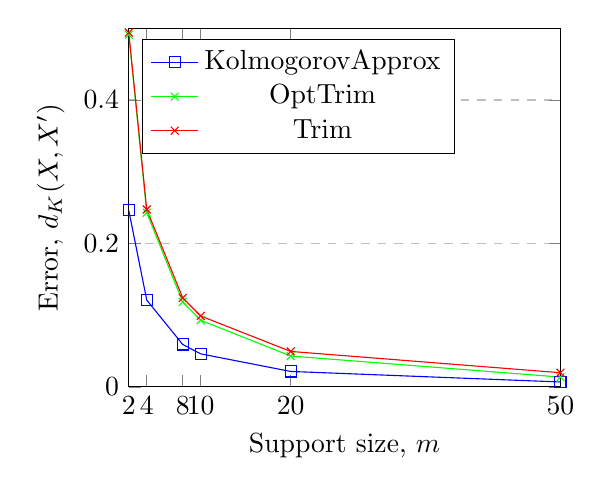
\begin{tikzpicture}
		\begin{axis}[
		scale=.8,
		xlabel={Support size, $m$},
		ylabel={Error, $d_K(X,X')$},
		xmin=2, xmax=50,
		ymin=0, ymax=0.5,
		xtick={2,4,8,10,20,50},
		legend pos=north west,
		ymajorgrids=true,
		grid style=dashed,
		]
		
		\addplot[
		color=blue,
		mark=square,
		]
		coordinates { 
			(2 , 0.246) 
			(4 , 0.121) 
			(8 , 0.0591) 
			(10 , 0.046) 
			(20, 0.0215) 
			(50, 0.0068) 
			
		};
		\addlegendentry{$\KlmApprox$}
		
		\addplot[
		color=green,
		mark=x,
		]
		coordinates {
			(2 , 0.491) 
			(4 , 0.2428) 
			(8 , 0.1184) 
			(10 , 0.0929) 
			(20, 0.0430) 
			(50, 0.0136) 
		};
		\addlegendentry{$\OptTrim$}
		
		\addplot[
		color=red,
		mark=x,
		]
		coordinates {
			(2 , 0.494) 
			(4 , 0.2473) 
			(8 , 0.124) 
			(10 , 0.0988) 
			(20, 0.0494) 
			(50, 0.01971)  
		};
		\addlegendentry{$\Trim$}
		
		\end{axis}
		\end{tikzpicture}
		\caption{Error comparison between $\KlmApprox$, $\OptTrim$, and $\Trim$, on randomly generated random variables as function of $m$.}
		\label{fig:error}
	\end{figure}
	
	
	\paragraph{Comparison to Linear Programming}
	
	We also compared the run-time of $\KlmApprox$ with a linear programing (LP) algorithm that also guarantees optimality, as described and discussed for example in~\cite{pavlikov2016cvar}.
	For that, we used the ``Minimize'' function of Wolfram Mathematica as a  state-of-the-art implementation of linear programing, encoding the problem by the LP problem $\min_{\alpha \in \mathbb{R}^n} \| x - \alpha\|_\infty$ subject to $\|\alpha\|_0 \leq m$ and $\| \alpha \|_1 =1$.
	The run-time comparison results were clear and persuasive: $\KlmApprox$ significantly outperforms the LP algorithm. For a random variable with support size $n=10$ and $m=5$, the LP algorithm run-time was $850$ seconds, where the $\KlmApprox$ algorithm run-time was less than a tenth of a second. For $n=100$ and $m=5$, the $\KlmApprox$ algorithm run-time was 0.14 seconds and the LP algorithm took more than a day. 
	Since it is not trivial to formally analyze the run-time of the LP algorithm, we conclude by the reported experiment that in this case the LP algorithm might not be as efficient as $\KlmApprox$ algorithm whose complexity is proven to be polynomial in Theorem~\ref{the:complexity}.
	
	\section{Discussion and future work}\label{sec:discussion}
	%Compact representations of distributions is mentioned in the literature in various contexts for various applications. In this paper, we are interested in finding optimal approximation of a random variables under the Kolmogorov metric which we define as optimal $m$-approximation. In order to achieve this optimal approximation two steps were taken, find the support of the optimal random variable and then calculate the pmf of each and every value in that support to minimize the error. Proofs of existences, optimality and run-time were detailed in Section~\ref{sec:alg} and the main algorithm was presented, the $\KlmApprox$ algorithm. Establishing the main contribution of this paper which is to present an optimal approximation scheme and to show it can be achieved in polynomial run-time. Furthermore, empirical evaluation was conducted on different domains and application to examine the algorithm performance in practice. We were interested in two aspects of performance - accuracy and run-time. Regarding to accuracy, as expected, the suggested $\KlmApprox$ algorithm results much smaller error compared to the other methods, sometimes, in more then factor 0f 2. Regarding to run-time, $\KlmApprox$ algorithm run-time is significantly much faster then LP approach. However, compared to other approximation methods accuracy vs. run-time is a trade off yet to be examined. Another interesting experiment that can be conducted in future work is to add the presented approach as one of the methods examined in~\cite{zeng2017comparison} and compare it to the binning approaches.
	
	We developed an algorithm for computing optimal approximations of random variables where the approximation quality is measured by the Kolmogorov distance.
	As demonstrated in the experiments, our algorithm improves on the approach of Cohen, Shimony and Weiss~\cite{cohen2015estimating} and~\cite{CohenGW18} in that it finds an optimal two sided Kolmogorov approximation, and not just one sided. Beyond the Kolmogorov measure studied here we believe that similar approaches may apply also to total variation, to the Wasserstein distance, and to other measures of approximations. Another direction for future work is extensions to tables that represent other objects, not necessarily random variables. To this end, we need to extend the algorithm to support tables that do not always sum to one and tables that may contain negative entries.
	
	
	\bibliography{library,Trim_Optimum}{}
	\bibliographystyle{abbrv}
	
\end{document}
